\documentclass{standalone}


\usepackage{tikz}
\usetikzlibrary{shapes,backgrounds,calc,patterns}
\usepackage{venndiagram}


\begin{document}
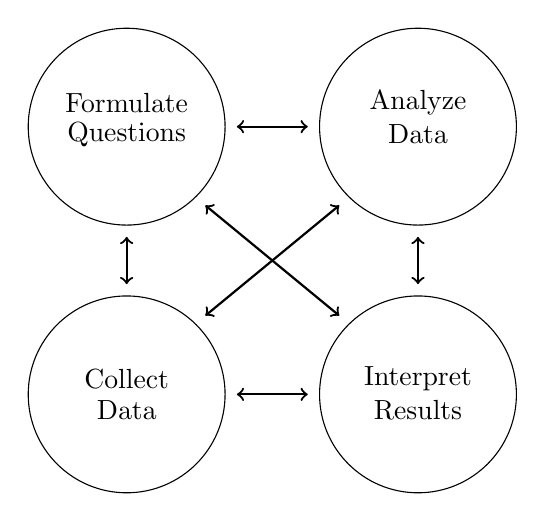
\begin{tikzpicture}
	%    \draw[step=1cm,gray,very thin] (-5,2.5) grid (5,-2.5);
	\draw (-4,1.4) circle (1.25);
	\node at (-4,1.7) {Formulate};
	\node at (-4,1.3) {Questions};

	
	\draw (-4,-2) circle (1.25);
	\node at (-4,-1.8) {Collect};
	\node at (-4,-2.2) {Data};

	
	\draw (-.3,1.4) circle (1.25);
	\node at (-.3,1.7) {Analyze};
	\node at (-.3,1.3) {Data};

	
	\draw (-.3,-2) circle (1.25);
	\node at (-.3,(-1.8) {Interpret};
	\node at (-.3,-2.2) {Results};

	

	
	\draw [<->,thick] (-2.6,1.4) -- (-1.7,1.4);
	\draw [<->,thick] (-2.6,-2) -- (-1.7,-2);
	\draw [<->,thick] (-4,0) -- (-4,-.6);
	\draw [<->,thick] (-3,-1) -- (-1.3,.4);
	\draw [<->,thick] (-.3,0) -- (-.3,-.6);
	\draw [<->,thick] (-1.3,-1) -- (-3,.4);

	
	\end{tikzpicture}
\end{document}